\documentclass[a4paper,12pt]{article}
\usepackage[utf8]{inputenc}
\usepackage{upquote}
\usepackage[margin=1in]{geometry} 
\usepackage{amsmath,amsthm,amssymb}
\usepackage{graphicx}     % for including graphics
\usepackage{caption}
\usepackage{hyperref}     % optional, for links
\usepackage{geometry}     % page geometry
\usepackage{listings}
\usepackage{algorithm}
\usepackage{placeins}
\usepackage{algpseudocode}
\newenvironment{statement}[2][Statement]{\begin{trivlist}
\item[\hskip \labelsep {\bfseries #1}\hskip \labelsep {\bfseries #2.}]}{\end{trivlist}}
\usepackage{xcolor}




\title{Assignment 4}

\begin{document}
\maketitle

\section{Introduction}

%Outlines the report.
%Contains information about contents, (research) questions and overall structure.

This report investigates the performance of the BFGS Quasi-Newton method combined with a strict (strong) Wolfe line search strategy for solving unconstrained optimization problems. The overarching goal is to assess:
\begin{itemize}
    \item Implement BFGS with a strict Wolfe condition line search.
    \item Evaluate its performance on various test functions, including high-dimensional problems.
    \item Compare our BFGS implementation with Newton's method and SciPy's BFGS.
    \item Analyze when BFGS is a competitive optimization method.
\end{itemize}

% The rest of the report is structured as follows: Section 2 provides the theoretical foundation, Section 3 describes the experimental setup, Section 4 presents results and discussion, and Section 5 concludes with key insights.


\section{Theory}

%Your Theoretical contributions.
%Theoretical considerations that shape choices in the experimental section.

\begin{enumerate}
    \item (Sufficient decrease / Armijo) 
    \[
       f(x_k + \alpha_k p_k) \;\le\; f(x_k) \;+\; c_1 \,\alpha_k\, \nabla f(x_k)^\top p_k
    \]
    \item (Strong curvature) 
    \[
       \bigl|\nabla f(x_k + \alpha_k p_k)^\top p_k\bigr| \;\le\; c_2\, \bigl|\nabla f(x_k)^\top p_k\bigr|\quad(0 < c_1 < c_2 < 1).
    \]
\end{enumerate}
Once a suitable $\alpha_k$ is found, we update $x_{k+1} = x_k + \alpha_k p_k$. Then define 
\[
s_k = x_{k+1} - x_k, \quad
y_k = \nabla f(x_{k+1}) - \nabla f(x_k),
\]
and update $H_k$ by the BFGS formula:
\[
   H_{k+1} \;=\; \bigl(I - \rho_k\, s_k y_k^\top\bigr)\,H_k \,\bigl(I - \rho_k\, y_k s_k^\top\bigr) \;+\; \rho_k\, s_k s_k^\top,
   \quad \text{where } \rho_k = \frac{1}{y_k^\top s_k}.
\]
Under suitable assumptions (e.g., $y_k^\top s_k > 0$) the matrix $H_k$ remains positive-definite, ensuring the search direction $p_k$ is indeed a descent direction.

\subsection{Theory problem 1}
\subsubsection*{SR1 Update Recap}
The Symmetric Rank-1 (SR1) update is a quasi-Newton scheme to approximate the Hessian (or its inverse). For a Hessian approximation $B_k$, the SR1 update is:
\[
  B_{k+1} 
  \;=\; 
  B_k 
  \;+\;
  \frac{\bigl(y_k - B_k \, s_k \bigr)\,\bigl(y_k - B_k \, s_k \bigr)^\top}
       {\bigl(y_k - B_k \, s_k \bigr)^\top \, s_k},
\]
where 
\[
  s_k = x_{k+1} - x_k, 
  \quad
  y_k = \nabla f(x_{k+1}) - \nabla f(x_k).
\]
Unlike BFGS, SR1 does not guarantee positive definiteness. Below, we see how it can become indefinite.

\subsubsection*{When SR1 is Indefinite}
If $(\,y_k - B_k\,s_k\,)^\top s_k < 0,$ the scalar in the denominator is negative, and
\[
  (\,y_k - B_k s_k\,)\,(y_k - B_k s_k)^\top
\]
is a rank-1 outer product that is positive semidefinite if multiplied by a positive scalar, but negative semidefinite if multiplied by a negative scalar. Hence, adding it to $B_k$ can introduce both positive and negative eigenvalues.  
\par
A simple case is $B_k = I$. Then,
\[
  B_{k+1} 
  = 
  I 
  + 
  \frac{(y_k - s_k)(y_k - s_k)^\top}{(y_k - s_k)^\top s_k}.
\]
If $(y_k - s_k)^\top s_k < 0,$ this term can shift $I$ sufficiently in directions where it becomes indefinite.  

\subsubsection*{2D Example with Wolfe Conditions}
In $\mathbb{R}^2$, pick $x_k$ and $x_{k+1}$ so that
\[
  (y_k)^\top s_k
  \quad
  \text{is small or negative compared to}
  \quad
  \|s_k\|^2
  \quad
  \text{and}
  \quad
  (y_k - s_k)^\top s_k<0.
\]
One can still satisfy the strong Wolfe conditions for the line search step going from $x_k$ to $x_{k+1}$. This shows that even when the line search is done carefully (via Wolfe), SR1 does not preserve positive definiteness. In practice, some implementations skip SR1 updates if the denominator is too small or negative to avoid losing definiteness.


\subsection{Theory problem 2}
\subsubsection*{Problem Statement}
Let
\[
  f(x) 
  = 
  \tfrac12 \, x^\top Q\,x 
  + 
  g^\top x,
\]
where $Q$ is symmetric positive definite. Suppose $B_k$ are positive-definite approximations such that $B_k \to Q$. We consider the iteration
\[
  x_{k+1} 
  = 
  x_k 
  - 
  B_k^{-1} \,\nabla f(x_k).
\]
We want to see why this yields superlinear convergence in $\|\nabla f(x_k)\|$.

\subsubsection*{Convergence Analysis}
Since $\nabla f(x) = Q\,x + g$, we have
\[
  \nabla f(x_{k+1})
  \;=\;
  Q\,x_{k+1} + g
  \;=\;
  \nabla f(x_k) 
  \;-\;
  Q\, B_k^{-1}\,\nabla f(x_k)
  \;=\;
  \bigl[I - Q\,B_k^{-1}\bigr]\,
  \nabla f(x_k).
\]
Define
\[
  R_k
  = 
  I - Q\,B_k^{-1}.
\]
Then
\[
  \nabla f(x_{k+1})
  =
  R_k\,\nabla f(x_k).
\]
If $B_k \to Q,$ then $B_k^{-1}\to Q^{-1},$ and hence $Q\,B_k^{-1}\to I,$ implying $R_k \to 0$. As $k\to\infty,$ $\|R_k\|\to 0.$ Therefore,
\[
  \|\nabla f(x_{k+1})\|
  =
  \| R_k\,\nabla f(x_k)\|
  \le
  \|R_k\|\,
  \|\nabla f(x_k)\|.
\]
Since $\|R_k\|\to 0,$ the ratio
\[
  \frac{\|\nabla f(x_{k+1})\|}{\|\nabla f(x_k)\|}
  \;\to\;
  0,
\]
which is the hallmark of superlinear (or faster) convergence. In the special case where $Q$ is constant and $B_k$ eventually becomes $Q$, you get exact Newton steps that solve the quadratic in finite steps.
\section{Experiments}

%Description of the experiments performed.
%Description of procedure and evaluation metrics.
%Also includes choices of parameters
\subsection{Implementation of BFGS}
\begin{algorithm}
\caption{BFGS Quasi-Newton Method}
\label{alg:BFGS}
\begin{algorithmic}[1]
\Require Objective function $f(x)$, gradient $\nabla f(x)$, initial guess $x_0$, tolerance $\epsilon$, maximum iterations $k_{\max}$.
\Ensure Approximate minimizer $x^*$.
\State Initialize: $x \gets x_0$, $H \gets I$ (identity matrix), $k \gets 0$
\State Compute initial gradient: $g \gets \nabla f(x)$
\While{$\| g \| > \epsilon$ \textbf{and} $k < k_{\max}$}
    \State Compute descent direction: $p \gets - H g$
    \State Perform line search to find step size $\alpha$ satisfying strict Wolfe conditions
    \State Update solution: $x_{\text{new}} \gets x + \alpha p$
    \State Compute new gradient: $g_{\text{new}} \gets \nabla f(x_{\text{new}})$
    \State Compute differences: $s \gets x_{\text{new}} - x$, $y \gets g_{\text{new}} - g$
    \If{$s^\top y > 0$} \Comment{Ensure curvature condition holds}
        \State Compute update factor: $\rho \gets \frac{1}{y^\top s}$
        \State Update Hessian approximation:
        \State $H \gets (I - \rho s y^\top) H (I - \rho y s^\top) + \rho s s^\top$
    \EndIf
    \State Update variables: $x \gets x_{\text{new}}, g \gets g_{\text{new}}, k \gets k + 1$
\EndWhile
\State \Return $x$
\end{algorithmic}
\end{algorithm}

\subsection{Evaluation Metrics}
\begin{itemize}
    \item \textbf{Iteration count}: Number of steps until convergence.
    \item \textbf{Function evaluations}: Cost in function/gradient calls.
    \item \textbf{Final function value} \( f(\mathbf{x}) \) and gradient norm \( \|\nabla f(\mathbf{x})\| \).
\end{itemize}
\subsection{Implementation Details}
\begin{itemize}
    \item \textbf{BFGS}: Uses strict Wolfe line search with parameters \( c_1 = 10^{-4}, c_2 = 0.9 \).
    \item \textbf{Newton}: Computes full Hessian and applies exact Newton steps.
    \item \textbf{SciPy BFGS}: Uses \texttt{scipy.optimize.minimize}.
\end{itemize}

\section{Results and Discussion}

%Presentation of the outcome of the experiments.
%Discussion of the results, including the knowledge gained from the theoretical questions.
%Also contains discussion of experimental shortcomings.

\begin{figure}[htbp]
    \centering
    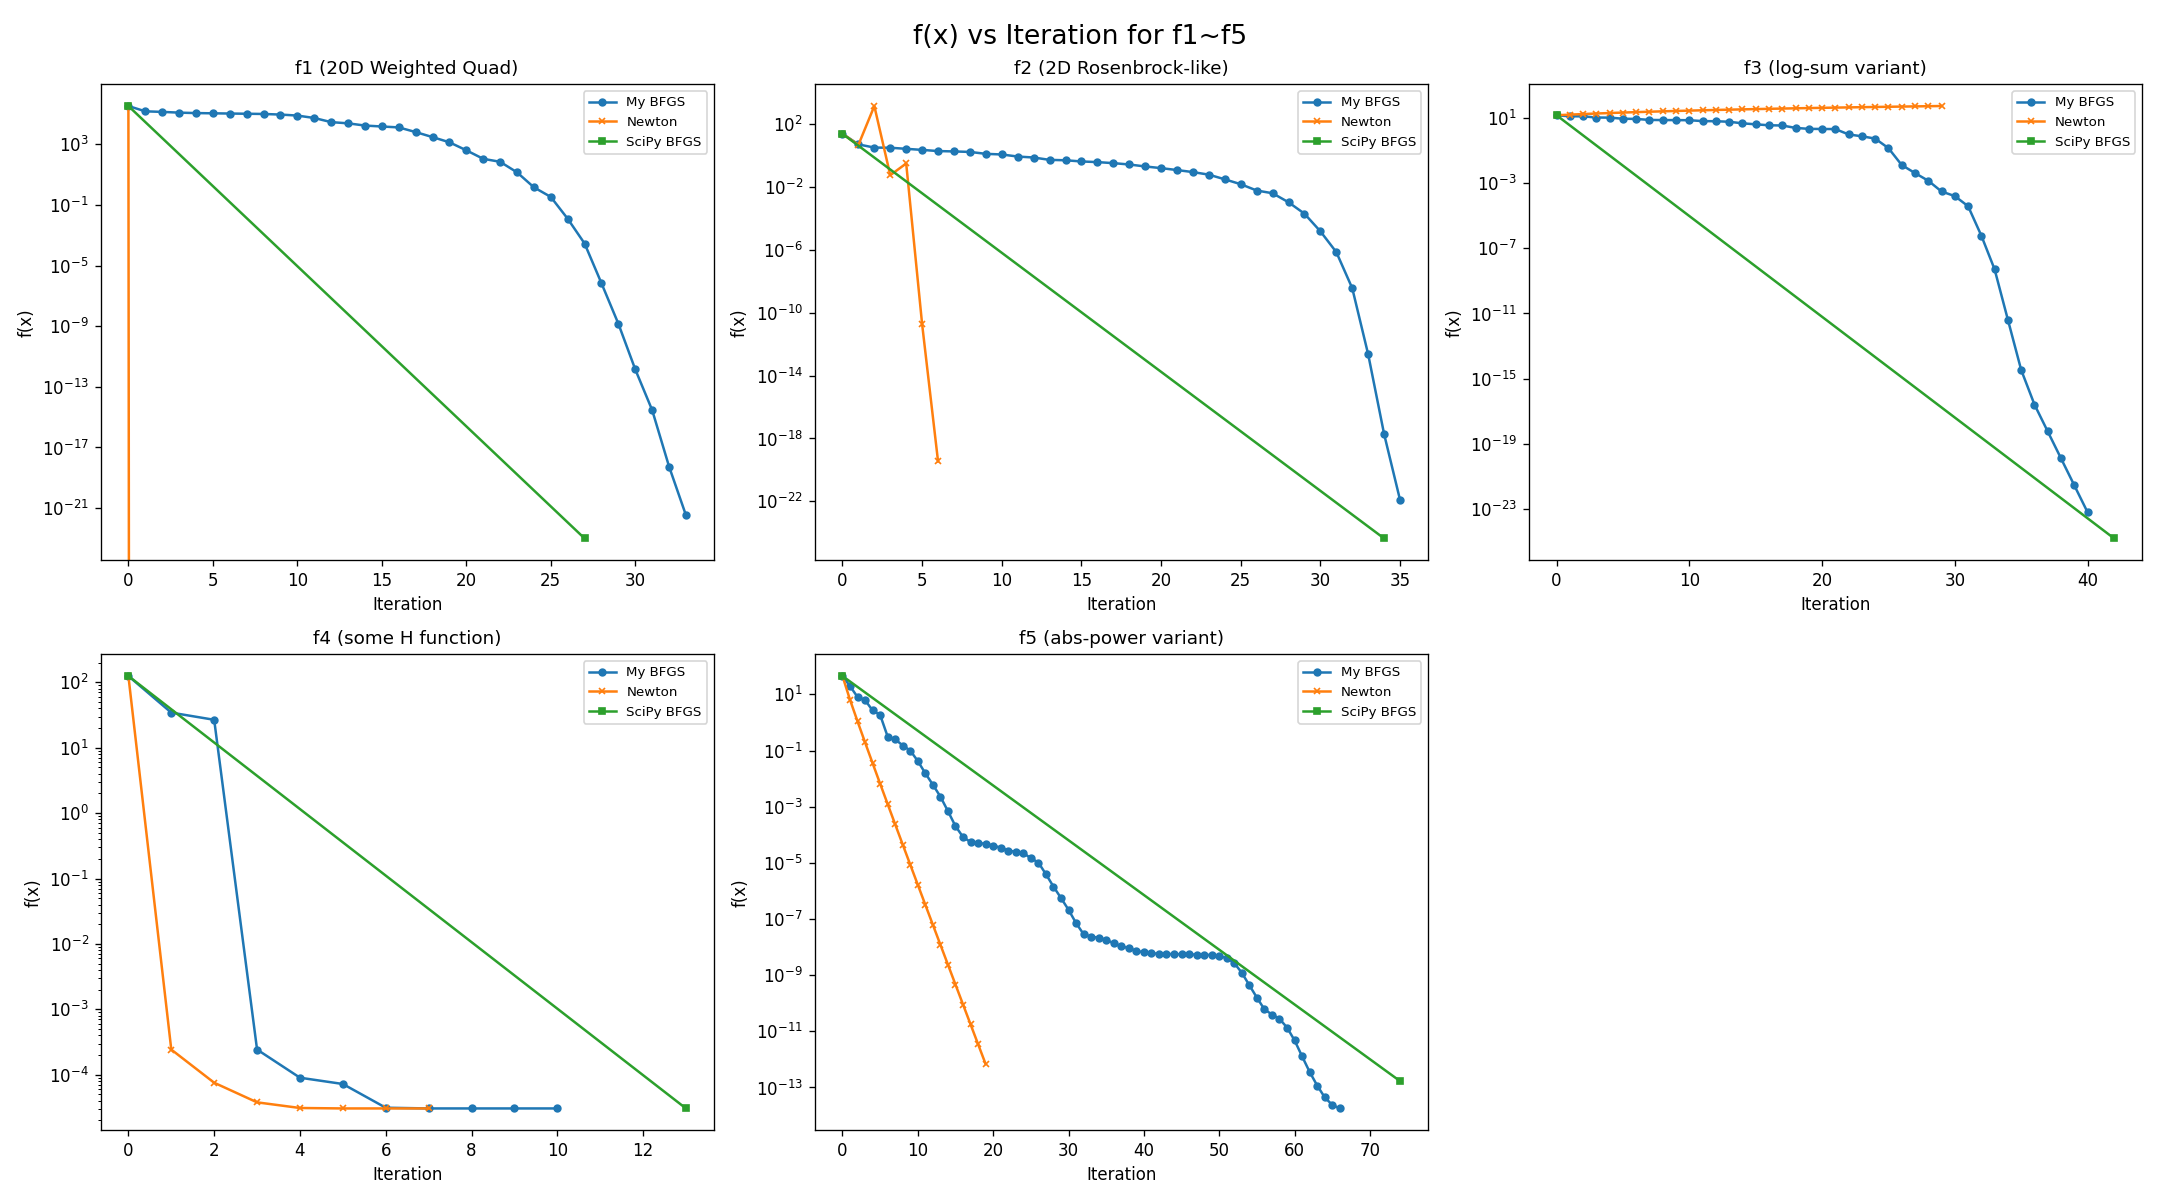
\includegraphics[width=0.82\linewidth]{pics/comparison_f_values.png}
    \caption{Convergence of function values for five test functions.}
    \label{fig:comparison-f}
\end{figure}
\begin{figure}[htbp]
    \centering
    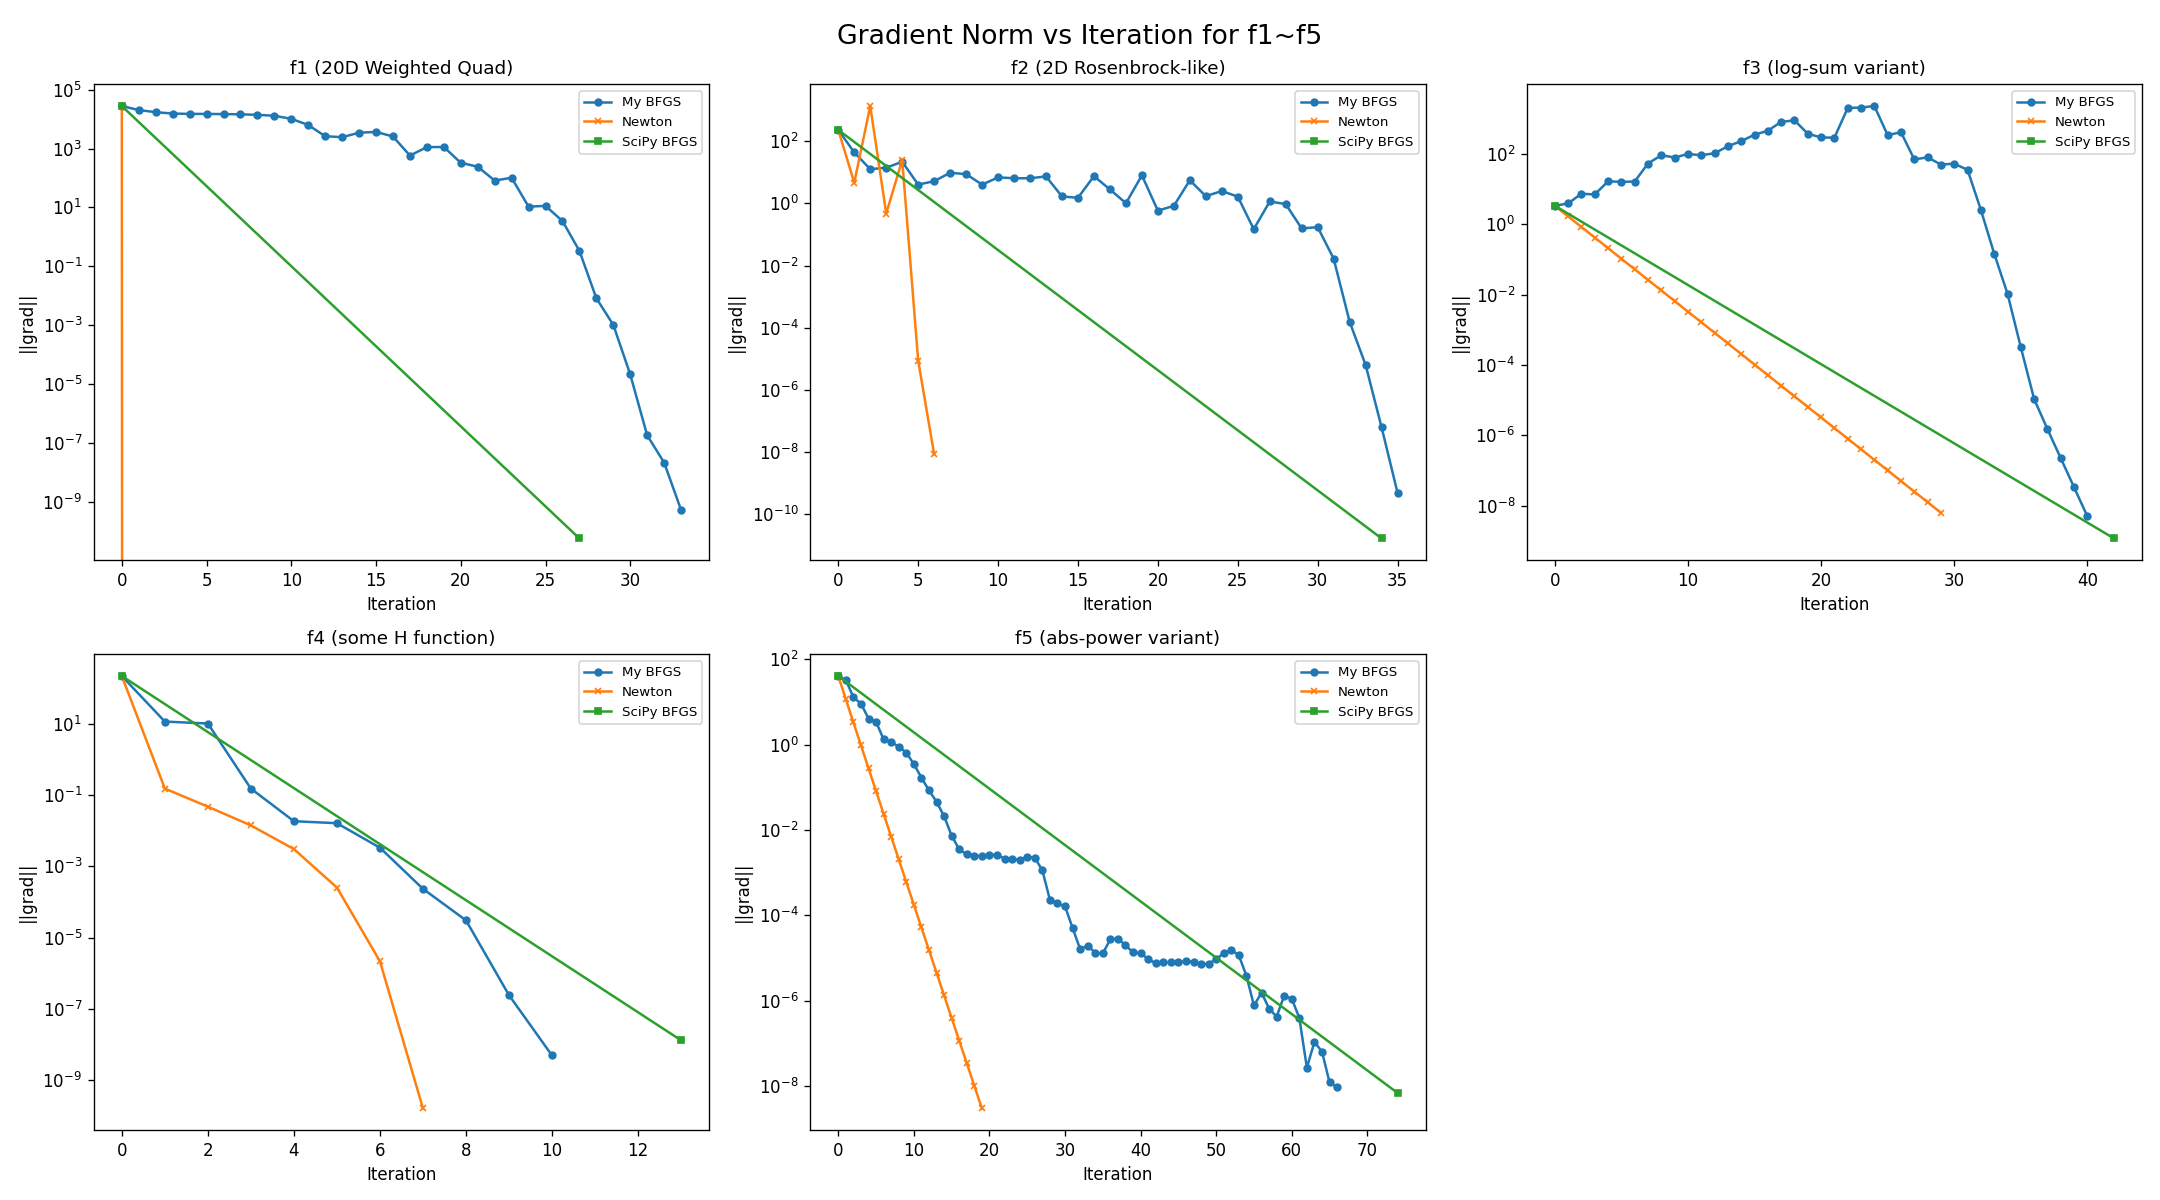
\includegraphics[width=0.82\linewidth]{pics/comparison_grad_norms.png}
    \caption{Convergence of gradient norms for five test functions.}
    \label{fig:comparison-grad}
\end{figure}
\subsection{Overall Performance}
From Figure \ref{fig:comparison-f} and Figure \ref{fig:comparison-grad}, we observe:
\begin{itemize}
    \item Newton's Method converges the fastest when the Hessian is computable and well-conditioned (e.g., f1, f2).
    \item BFGS performs well for high-dimensional problems and avoids expensive Hessian computations.
    \item SciPy BFGS generally converges faster than our implementation but follows a similar trend.
\end{itemize}

\subsection{Function-Specific Observations}
\begin{itemize}
    \item \textbf{f1}: Newton converges in 1 step; BFGS takes 33 steps.
    \item \textbf{f2}: Newton converges in 6 steps; BFGS takes 35.
    \item \textbf{f3}: Newton fails to reach a good solution due to Hessian instability, whereas BFGS reaches $10^{-24}$.
    \item \textbf{f4}: All methods achieve similar final function values.
    \item \textbf{f5}: BFGS converges faster than SciPy BFGS.
\end{itemize}

\subsection{Discussion}
Newton's method is fastest when Hessian is easy to compute. BFGS is more practical for medium-to-high-dimensional problems. SciPy’s BFGS shows slight advantages in some cases. In non-convex problems (e.g., f3), BFGS is more stable than Newton. BFGS is an alternative when the Hessian is not available or is computationally expensive. In high-dimensional optimization problems, BFGS has lower computational complexity and only requires first-order gradient information for each update, making it suitable for large-scale optimization problems. It converges slightly slower than Newton, but much faster than first-order gradient descent.


\section{Conclusion}

%What knowledge have we gained?
%5Could we answer the question we set out to answer in the Introduction?
Overall, implementing BFGS with a strict Wolfe line search demonstrates effective convergence for a wide range of test functions, often matching or closely trailing the performance of Newton’s method (where Hessian computation is viable) and SciPy’s official BFGS. For simple or low-dimensional problems with an easily computed Hessian, Newton’s method is typically faster. Our results confirm that BFGS’s approximate Hessian updates, paired with a proper line search, achieve stable convergence and maintain numerical efficiency across various test cases.

\end{document}
